
% THESIS INTRODUCTION

\chapter{Introduction}
\label{chap:introduction}
\ifpdf
    \graphicspath{{Introduction/Figures/PNG/}{Introduction/Figures/PDF/}{Introduction/Figures/}}
\else
    \graphicspath{{Introduction/Figures/EPS/}{Introduction/Figures/}}
\fi

% short summary of the chapter
\section*{Summary}

This Chapter will introduce  the reader to the topic of this master thesis. It will present the problem statement and the followed work plan.

\section{Overview}

In the latest years, aerial robotics has grown so fast both in technology and popularity among the public and multirotor aircrafts such as quadcopters are one of the most promising fields. In fact those type of vehicles have become a standard platform for research in many laboratories , driven by totally different customer needs the research improved substantially. They have sufficient payload and flight endurance to support a number of indoor and outdoor applications, and the improvements of battery and other technology is rapidly increasing the scope for commercial opportunities. They are highly maneuverable and enable safe and low-cost experimentation in mapping, navigation, and control strategies for robots that move in three-dimensional space. Small quadrotors have been demonstrated for exploring and mapping 3-D environments; transporting, manipulating, and assembling objects; and acrobatic tricks such as juggling, balancing, and flips. \\*

\begin{figure}[h]
\centering
 \noindent
 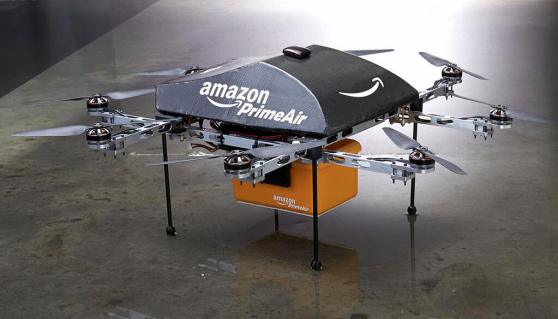
\includegraphics[width=0.4\textwidth]{amazon.jpg}\hspace{0.1\textwidth}
 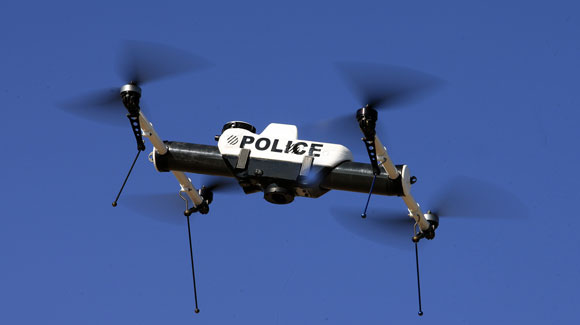
\includegraphics[width=0.4\textwidth]{police-drone.jpg}\\[2em]
 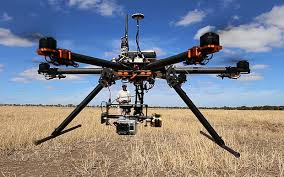
\includegraphics[width=0.4\textwidth]{gopro.jpg}\hspace{0.1\textwidth}
 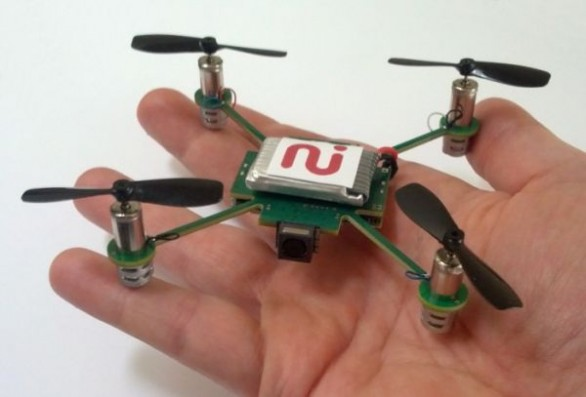
\includegraphics[width=0.4\textwidth]{microcopter.jpg}\par
 \caption{Different applications of multirotors}
 \label{figure:applications}
\end{figure}

\noindent
As stated before, the uses of this platform are many and limited
only by the imagination of the designers. Figure \ref{figure:applications} illustrates various application going from search and rescue to public defense, most of them in outdoor scenarios. Very interesting is to investigate the possible use of this technology in an indoor scene where the comforting signal of the GPS is not present and analyze every aspect of flight going from state estimation, control and stability to autonomy, path planning and high level automation. \\*

This work investigates the integration between different heterogeneous entities as well as the possibility to design a safe, reliable and flexible architecture capable of letting the robot navigate safely in an indoor environment. At the end a simple algorithm for landing on a mobile platform is presented with very interesting results demonstrating the potential of this setup.

\subsection{Hosting laboratories}
This thesis is carried out as a cooperation between the Laboratorium Lab (focus:
autonomous robotics and ambient intelligence), the NOCC Lab (focus: control,
identification and estimation) and the EMARO@DIBRIS Lab.

\newpage

\section{Problem statement}

The goal of this master thesis to develop algorithms for UAV trajectory planning and execution (as well as the related SW components), using the motion capture system as the source of the UAV position feedback. Once achieved stability more complex aspects are investigated, a task based software architecture is presented and a simple technique for landing on a mobile platform is proposed.
The above stated, is formulated in to the following problem statement for the project: \\*

\noindent
\textit{We want to design a set of algorithms and SW components enabling a quadrotor to achieve stability, through position feedback given from a motion capture system, and perform different tasks in an indoor scenario. }

\subsection{Work plan}
The work got through several tasks covering all aspects, they can be distinctly divided in main blocks hence defining the work plan.

\begin{enumerate}

\item Analysis of state of the art approaches to UAV control, modeling, trajectory planning and execution

\item Technical analysis and documentation on the given tools (Autopilot, Motion Capture, IRIS Quadcopter)

\item Integration between mocap and IRIS
\begin{itemize}

\item Integration and testing between mocap and onboard estimation modules
\item Integration and testing of onboard controller through set point control

\end{itemize}

\item Design of the high level software architecture 
\item Testing the software, coding and debugging different kind of tasks
\item Design and testing an algorithm for landing on a mobile platform

\end{enumerate}

\subsection{Thesis structure}
The thesis presents procedures, techniques, comments and results obtained during the work. The document is divided in chapters dedicated to particular aspects of the project, the structure is the following: 

\paragraph{Chapter 2} Synthesizes the preliminary literature review explaining existing research, products and systems and analyzes some robotics platforms and tools. A suitable modeling technique for this kind of vehicles is described introducing additional non linearities and explaining when the model uses them.
Moreover it introduces a survey on various control techniques that are currently used highlighting pros and cons. At the end some comments are given about software architecture trends which are used in this field. 


\paragraph{Chapter 3}

This chapter introduces the reader the current laboratory setup illustrating which kind of tools are used as well as the specifications of each component. Then it presents the integration both at hardware and software levels of each part of the system. 

\paragraph{Chapter 4}
This part concerns the modeling of the IRIS quad rotor. A model of the quadrotor is necessary to develop a controller and understand better its dynamics. The first part presents some generalities including the reference frames used in order to define the world and the robot. It also contains a list of assumptions done to simplify the model. After, the involved physical principles and the actual derivation of the model are explained.

\paragraph{Chapter 5}

This chapter presents the techniques that are used to estimate the system's states and to stabilize the IRIS robot which are currently implemented in the PX4 Firmware. After a quick overview of the estimator modules, the controller architecture is presented. Moreover, this chapter explains in details how the on board autopilot interfaces with the software architecture and which modules are involved.

\paragraph{Chapter 6}

This Chapter introduces the reader to the software architecture running off board on Linux. The introduction presents a  general overview on software architectures, expresses the needs of such a system and in particular it describes the environment and software tools involved. Next section presents the design pattern according to which the software is organized explaining its advantages and limitations. Then the software components are described with more detail one by one and the results of the experiments are reported. 


\paragraph{Chapter 7}

This chapter concerns with the task of landing on a platform of arbitrary height while it is moving on the horizontal plane. After a brief introduction to the topic and the statement of general assumptions, the experimental setup is described. Later on the solution to the problem is presented and the control algorithm described. Last section presents and comments experiment results.

\paragraph{Chapter 8}

The last chapter presents the conclusions of this work. It highlights the most relevant steps and summarizes what has been done. Then it points out what could be improved and gives a number of ideas relating the future work.










